\begin{frame}{\og{}Napoléon des névroses\fg{} ou \og{}Paganini de l'hystérie\fg{} {\small(\hypersetup{citecolor=yellow}\cite{marmion2015freud})}}

\textsc{\textcolor{deepblue}{\textbf{Jean-Martin CHARCOT}} (1825-1893)}
%\hbox{\hspace{25em} 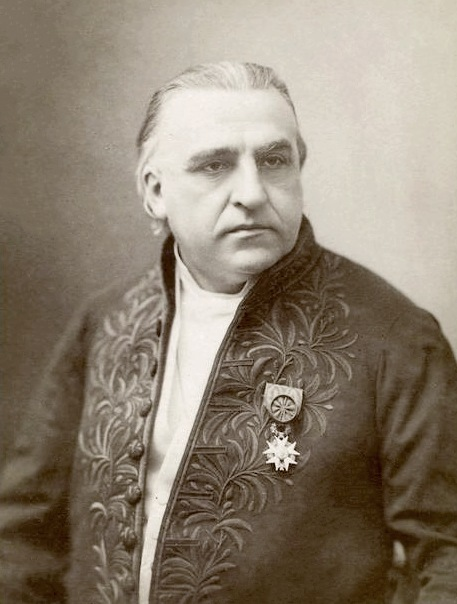
\includegraphics[scale=0.07]{pic/Jean-Martin_Charcot.jpg}}
%\\{\scriptsize Portrait de\\Charcot (\href{https://fr.wikipedia.org/wiki/Jean-Martin_Charcot}{Wikipedia}).}
\hbox{\hspace{10.3em} 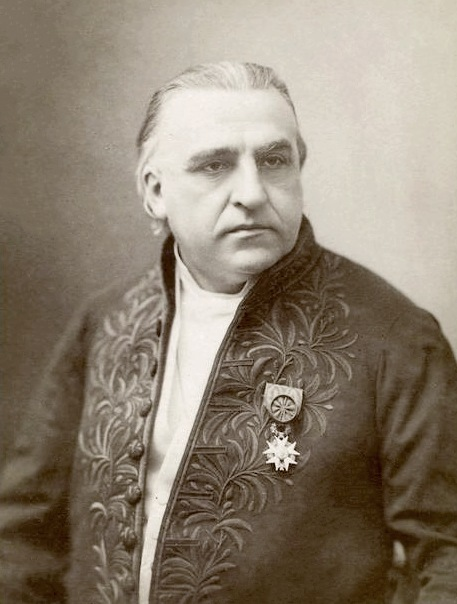
\includegraphics[scale=0.06]{pic/Jean-Martin_Charcot.jpg}}\\\hbox{\hspace{23.8em}{\tiny Source : \href{https://fr.wikipedia.org/wiki/Jean-Martin_Charcot}{Wikipedia}}.}
\begin{itemize}
\item père de la neurologie moderne et française au XIX\ieme{} s. 
\item leçons cliniques du mardi à l'hôpital de la Salpêtrière à Paris \\
\hspace{165pt}
\footnotesize\og{}Mecque de la neurologie\fg{}
\end{itemize}
\begin{enumerate}[\indent {}]
\item Contributions majeures :
\begin{table}[h!]
\small
\begin{tabular}{l l}
\textcolor{darkgray}{hystérie} & $\leftarrow$ lésion dynamique des circuits cérébraux\\
\textcolor{darkgray}{hypnose} & analyse et traitement des symptômes hystériques\\
\textcolor{darkgray}{SEP} & description de la \textit{sclérose en plaques} disséminée\\
\textcolor{darkgray}{SLA} & description de la \textit{sclérose latérale amyotrophique}\\
\textcolor{darkgray}{maladie de Parkinson} & concepteur du terme (avec A. Vulpian)
\end{tabular}
\end{table}
%	\begin{description}
%	    \item[hystérie] 
%	    résultat d'une lésion dynamique des circuits cérébraux
%    \item[hypnose] 
%    analyse des symptômes hystériques et outil thérapeutique
%    \item[SEP]\footnote{abbr. \textit{sclérose en plaques}.}
%     disséminée (description) $\rightarrow$ sclérose multiple
%    \item[SLA]\footnote{abbr. \textit{sclérose latérale amyotrophique}.}
%     (description) $\rightarrow$ maladie de Charcot / Lou Gehrig
%    \item[maladie de Parkinson]
%    concepteur du terme (avec A. Vulpian)
%	\end{description}  
	\end{enumerate}
	\vspace{-0.3cm}
    % \item hystérie est due à une \textit{lésion dynamique} de l’encéphale, liée à un traumatisme de nature physique (accident de train, chute, choc$\dots$) -- possible de recréer sous hypnose
    % \item impact sur les acteurs dans ou en dehors de sa discipline : S. Freud, G. de la Tourette, E. Zola$\dots$
    \begin{flushright}
{\footnotesize(\cite{camargo2024jean})}
\end{flushright}

%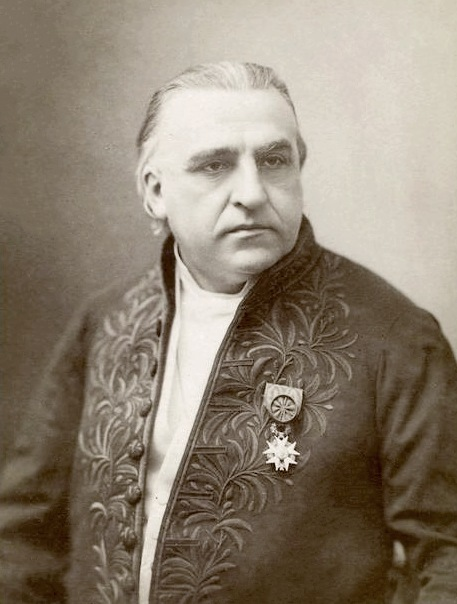
\includegraphics[width=10pt]{pic/Jean-Martin_Charcot.jpg}%
%\\{\scriptsize Portrait de\\Charcot (\href{https://fr.wikipedia.org/wiki/Jean-Martin_Charcot}{Wikipedia}).}



\end{frame}

\begin{frame}{Impact de Charcot sur sa discipline et au-delà}
\centering
\textbf{Collaborateurs et élèves}\\
{\small \og{}réseau scientifique\fg{}}
    \begin{table}[!ht]
        \centering
        \small
        \begin{tabular}{l r}
           Sigmund \textsc{Freud} (1856-1939)  & théorie psychanalytique \\
            Gilles \textsc{de la Tourette} (1857-1932) & syndrôme de Tourette \\
            Joseph \textsc{Babinski} (1857-1904) & pithiatisme, signe de Babinski \\
%           Pierre \textsc{Janet} (1859-1947) & psychopathologie
%            dissociation, sous-conscient 
        \end{tabular}
        \begin{flushright}
%        \footnotesize\citep{bogousslavsky2020}
        \footnotesize\citep{BROUSSOLLE2012301}
        \end{flushright}
        % \caption{Caption}
        \label{tab:my_label}
    \end{table}
\medskip
\textbf{Écrivains naturalistes français et européens} 
\begin{itemize}
\centering
\small \item références à Charcot et aux descriptions de crises hystériques
\end{itemize}
\begin{table}[!ht]
    \centering
    \small
    \begin{tabular}{l r}
        Émile \textsc{Zola} (1840–1902)  & \textit{Lourdes} \\
        Léon \textsc{Tolstoï} (1828–1910) & \textit{La Sonate à Kreutzer} \\
        Luigi \textsc{Capuana} (1839–1915) & \textit{La Torture}
%        Bjørnstjerne \textsc{Bjørnson} (1832–1910) & \textit{Over Ævne}
    \end{tabular}
            \begin{flushright}
        \footnotesize\citep{koehler2013charcot}
        \end{flushright}
    % \caption{Caption}
    \label{tab:my_label}
\end{table}

\end{frame}

\begin{frame}{Question de recherche}
% Comment mesurer le degré d'intertextualité entre Charcot et son réseau scientifique et artistique au prisme du numérique ?
% create the main block
\begin{exampleblock}{}
\centering
    \color{deepblue}{\textmd{Comment mesurer le degré d'intertextualité entre Charcot et son réseau scientifique au prisme du numérique ?}}
\end{exampleblock}

\end{frame}
